% Options for packages loaded elsewhere
\PassOptionsToPackage{unicode}{hyperref}
\PassOptionsToPackage{hyphens}{url}
\PassOptionsToPackage{dvipsnames,svgnames,x11names}{xcolor}
%
\documentclass[
  9pt,
  letterpaper,
  DIV=11,
  numbers=noendperiod]{scrartcl}

\usepackage{amsmath,amssymb}
\usepackage{iftex}
\ifPDFTeX
  \usepackage[T1]{fontenc}
  \usepackage[utf8]{inputenc}
  \usepackage{textcomp} % provide euro and other symbols
\else % if luatex or xetex
  \usepackage{unicode-math}
  \defaultfontfeatures{Scale=MatchLowercase}
  \defaultfontfeatures[\rmfamily]{Ligatures=TeX,Scale=1}
\fi
\usepackage{lmodern}
\ifPDFTeX\else  
    % xetex/luatex font selection
  \setmainfont[]{Times New Roman}
\fi
% Use upquote if available, for straight quotes in verbatim environments
\IfFileExists{upquote.sty}{\usepackage{upquote}}{}
\IfFileExists{microtype.sty}{% use microtype if available
  \usepackage[]{microtype}
  \UseMicrotypeSet[protrusion]{basicmath} % disable protrusion for tt fonts
}{}
\makeatletter
\@ifundefined{KOMAClassName}{% if non-KOMA class
  \IfFileExists{parskip.sty}{%
    \usepackage{parskip}
  }{% else
    \setlength{\parindent}{0pt}
    \setlength{\parskip}{6pt plus 2pt minus 1pt}}
}{% if KOMA class
  \KOMAoptions{parskip=half}}
\makeatother
\usepackage{xcolor}
\usepackage[margin=1in]{geometry}
\setlength{\emergencystretch}{3em} % prevent overfull lines
\setcounter{secnumdepth}{-\maxdimen} % remove section numbering
% Make \paragraph and \subparagraph free-standing
\ifx\paragraph\undefined\else
  \let\oldparagraph\paragraph
  \renewcommand{\paragraph}[1]{\oldparagraph{#1}\mbox{}}
\fi
\ifx\subparagraph\undefined\else
  \let\oldsubparagraph\subparagraph
  \renewcommand{\subparagraph}[1]{\oldsubparagraph{#1}\mbox{}}
\fi


\providecommand{\tightlist}{%
  \setlength{\itemsep}{0pt}\setlength{\parskip}{0pt}}\usepackage{longtable,booktabs,array}
\usepackage{calc} % for calculating minipage widths
% Correct order of tables after \paragraph or \subparagraph
\usepackage{etoolbox}
\makeatletter
\patchcmd\longtable{\par}{\if@noskipsec\mbox{}\fi\par}{}{}
\makeatother
% Allow footnotes in longtable head/foot
\IfFileExists{footnotehyper.sty}{\usepackage{footnotehyper}}{\usepackage{footnote}}
\makesavenoteenv{longtable}
\usepackage{graphicx}
\makeatletter
\def\maxwidth{\ifdim\Gin@nat@width>\linewidth\linewidth\else\Gin@nat@width\fi}
\def\maxheight{\ifdim\Gin@nat@height>\textheight\textheight\else\Gin@nat@height\fi}
\makeatother
% Scale images if necessary, so that they will not overflow the page
% margins by default, and it is still possible to overwrite the defaults
% using explicit options in \includegraphics[width, height, ...]{}
\setkeys{Gin}{width=\maxwidth,height=\maxheight,keepaspectratio}
% Set default figure placement to htbp
\makeatletter
\def\fps@figure{htbp}
\makeatother

\KOMAoption{captions}{tableheading}
\usepackage{graphicx}
\usepackage{fancyhdr}
\pagestyle{fancy}
\fancyhead[L]{Module 1 – Raising Equity Capital}
\fancyhead[R]{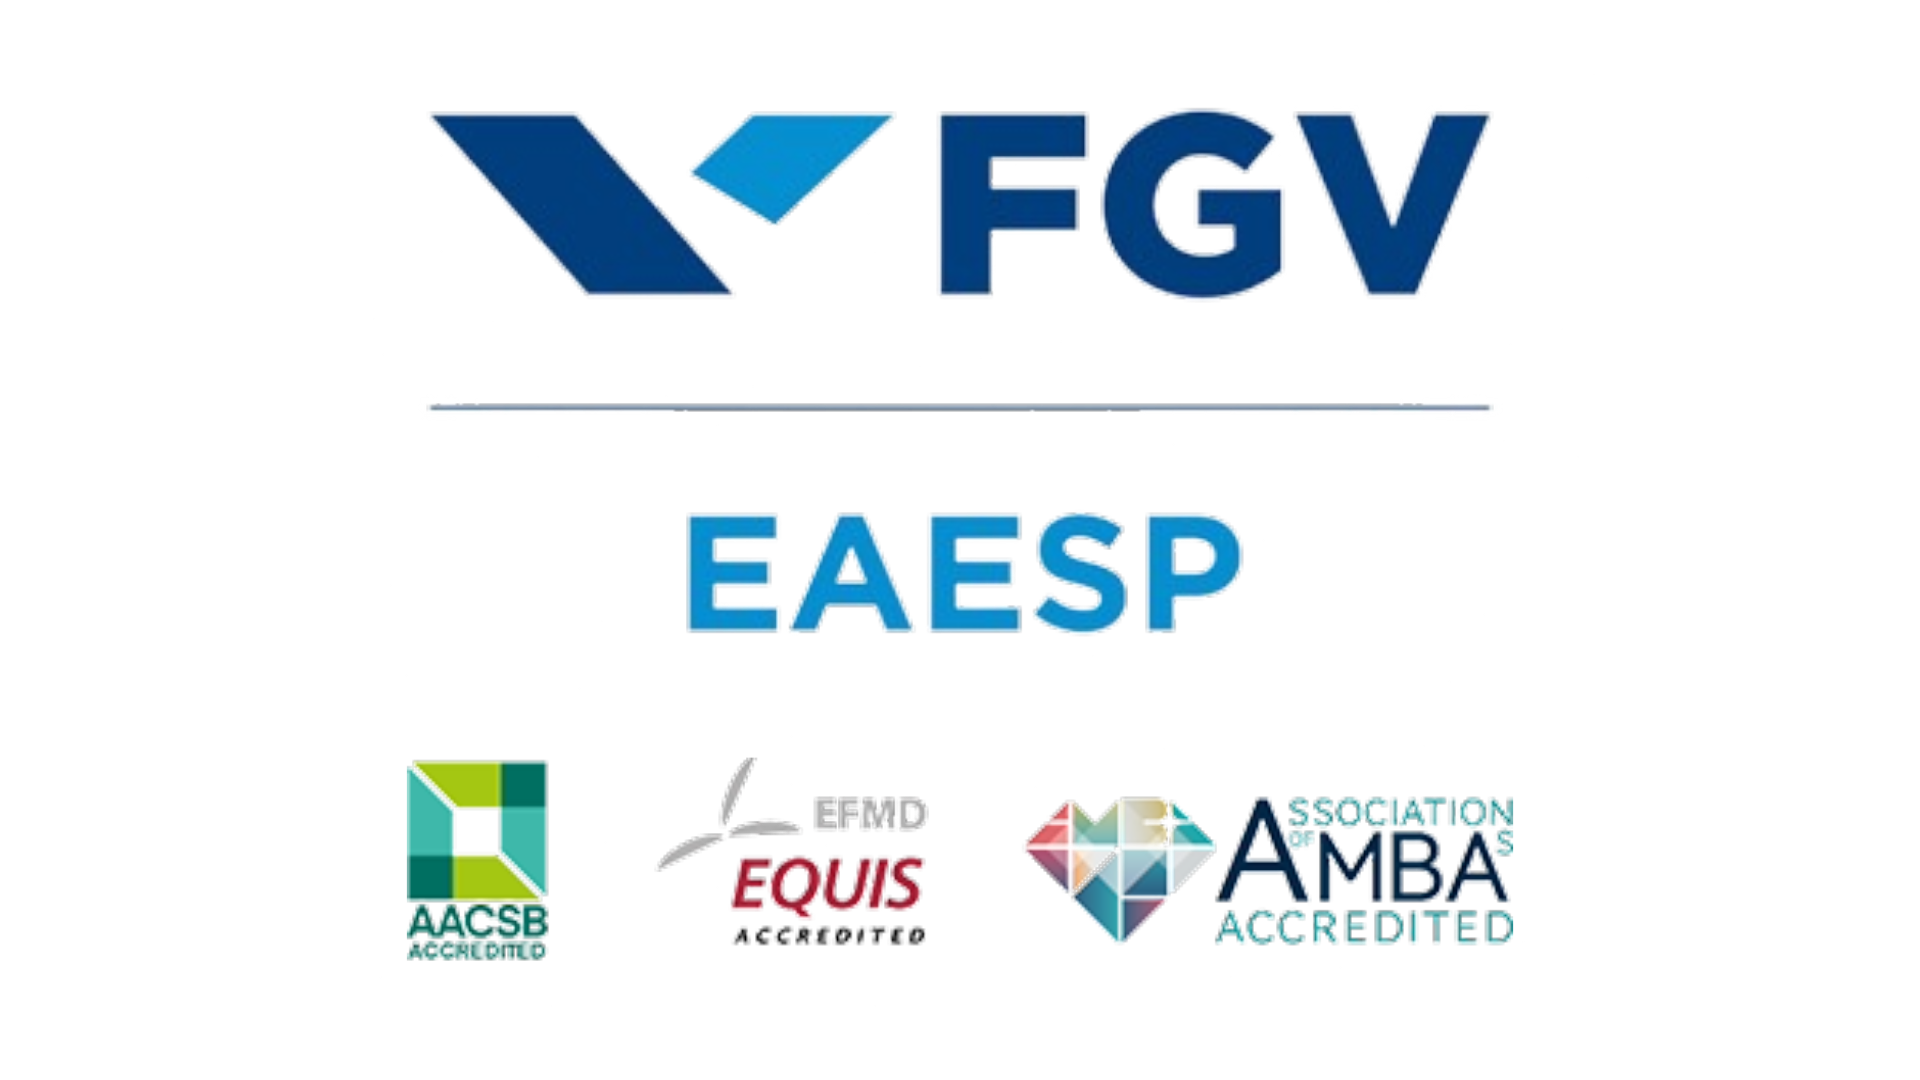
\includegraphics[height=1.2cm]{../figs/background8.png}}
\fancyfoot[C]{}
\makeatletter
\@ifpackageloaded{caption}{}{\usepackage{caption}}
\AtBeginDocument{%
\ifdefined\contentsname
  \renewcommand*\contentsname{Table of contents}
\else
  \newcommand\contentsname{Table of contents}
\fi
\ifdefined\listfigurename
  \renewcommand*\listfigurename{List of Figures}
\else
  \newcommand\listfigurename{List of Figures}
\fi
\ifdefined\listtablename
  \renewcommand*\listtablename{List of Tables}
\else
  \newcommand\listtablename{List of Tables}
\fi
\ifdefined\figurename
  \renewcommand*\figurename{Figure}
\else
  \newcommand\figurename{Figure}
\fi
\ifdefined\tablename
  \renewcommand*\tablename{Table}
\else
  \newcommand\tablename{Table}
\fi
}
\@ifpackageloaded{float}{}{\usepackage{float}}
\floatstyle{ruled}
\@ifundefined{c@chapter}{\newfloat{codelisting}{h}{lop}}{\newfloat{codelisting}{h}{lop}[chapter]}
\floatname{codelisting}{Listing}
\newcommand*\listoflistings{\listof{codelisting}{List of Listings}}
\makeatother
\makeatletter
\makeatother
\makeatletter
\@ifpackageloaded{caption}{}{\usepackage{caption}}
\@ifpackageloaded{subcaption}{}{\usepackage{subcaption}}
\makeatother
\ifLuaTeX
  \usepackage{selnolig}  % disable illegal ligatures
\fi
\usepackage{bookmark}

\IfFileExists{xurl.sty}{\usepackage{xurl}}{} % add URL line breaks if available
\urlstyle{same} % disable monospaced font for URLs
\hypersetup{
  pdftitle={Module 1 -- Raising Equity Capital},
  pdfauthor={Henrique C. Martins},
  colorlinks=true,
  linkcolor={blue},
  filecolor={Maroon},
  citecolor={Blue},
  urlcolor={Blue},
  pdfcreator={LaTeX via pandoc}}

\title{Module 1 -- Raising Equity Capital}
\author{Henrique C. Martins}
\date{}

\begin{document}
\maketitle

\subsection{Core Concepts}\label{core-concepts}

\subsubsection{1. Equity for Private
Companies}\label{equity-for-private-companies}

Private firms often rely on angel investors or venture capital (VC) to
grow. Angels invest early using SAFEs or convertible notes. VCs raise
capital from institutions, offer expertise, and demand strong control.
Private equity targets mature firms via leveraged buyouts. Corporate and
institutional investors bring strategic goals or diversification.

\begin{center}\rule{0.5\linewidth}{0.5pt}\end{center}

\subsubsection{2. Raising Capital: From VC to
IPO}\label{raising-capital-from-vc-to-ipo}

Startups issue preferred stock---convertible, no dividends, senior in
liquidation. Each funding round (e.g., Series A) sets new terms.
Valuation is split into \textbf{pre-money} (before investment) and
\textbf{post-money} (after). Founders are diluted over time.

An \textbf{IPO} provides liquidity and new capital but demands
transparency. Underwriters manage the offering, price via \textbf{book
building}, and charge fees (\textasciitilde7\%). IPOs tend to be
underpriced and cyclical; long-term performance is mixed.

\begin{center}\rule{0.5\linewidth}{0.5pt}\end{center}

\subsubsection{3. Seasoned Equity Offerings
(SEO)}\label{seasoned-equity-offerings-seo}

Public firms may issue equity again via SEOs. In a \textbf{cash offer},
new shares are sold broadly. In a \textbf{rights offer}, only current
shareholders may buy. Rights offers prevent dilution. SEOs can trigger
negative price reactions and still carry costs (\textasciitilde5\%).

\begin{center}\rule{0.5\linewidth}{0.5pt}\end{center}

\begin{center}

\includegraphics[height=1.3cm]{../figs/background6.png}
\end{center}

\begin{center}
\includegraphics[width=1.8cm]{https://api.qrserver.com/v1/create-qr-code/?size=80x80&data=https://henriquemartins.net/teaching/financial_strategy/module1/p1.html}
\includegraphics[width=1.8cm]{https://api.qrserver.com/v1/create-qr-code/?size=80x80&data=https://henriquemartins.net/teaching/financial_strategy/p1tf.html}
\includegraphics[width=1.8cm]{https://api.qrserver.com/v1/create-qr-code/?size=80x80&data=https://henriquemartins.net/teaching/financial_strategy/p1num.html}
\includegraphics[width=1.8cm]{https://api.qrserver.com/v1/create-qr-code/?size=80x80&data=https://henriquemartins.net/teaching/financial_strategy/p1mcq.html}
\includegraphics[width=1.8cm]{https://api.qrserver.com/v1/create-qr-code/?size=80x80&data=https://henriquemartins.net/teaching/financial_strategy/p1long.html}
\end{center}

\begin{center}
{\footnotesize Slides | T/F | Numeric | MCQ | Long-form}
\end{center}



\end{document}
